\documentclass[border=3pt,tikz]{standalone}
\usepackage{amsmath}
\usetikzlibrary{calc}
\usetikzlibrary{arrows.meta} % for arrow size
\begin{document}
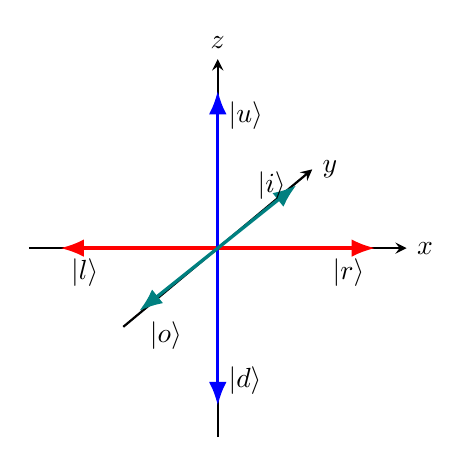
\begin{tikzpicture}[scale=2]

    
    \draw[thick,->,>=stealth] (-1.2, 0) -- (1.2, 0) node[right] {$x$};
    \draw[thick,->,>=stealth] (-0.6, -0.5) -- (0.6, 0.5) node[right] {$y$};
    \draw[thick,->,>=stealth] (0, -1.2) -- (0, 1.2) node[above] {$z$};
    
    \draw [very thick, red, -{Latex[length=3mm]}] (0,0) -- (1,0) node [below left, black] {$|r\rangle$};
    \draw [very thick, red, -{Latex[length=3mm]}] (0,0) -- (-1,0) node [below right, black] {$|l\rangle$};
    \draw [very thick, blue, -{Latex[length=3mm]}] (0,0) -- (0,1) node [below right, black] {$|u\rangle$};
    \draw [very thick, blue, -{Latex[length=3mm]}] (0,0) -- (0,-1) node [above right, black] {$|d\rangle$};
    \draw [very thick, teal, -{Latex[length=3mm]}] (0,0) -- (0.5,0.4) node [left, black] {$|i\rangle$};
    \draw [very thick, teal, -{Latex[length=3mm]}] (0,0) -- (-0.5,-0.4) node [below right, black] {$|o\rangle$};
    
    \end{tikzpicture}
    \end{document}